\FloatBarrier
\section{Elementos de instalación}\label{sec:instalacion}

\subsection{Lista de materiales de la estructura de montaje}

Los 374 módulos se distribuyen en 22 filas de este a oeste, con 17 módulos en posición vertical por fila, inclinados \SI{10}{\degree} hacia el sur. Las filas se colocan paralelas al borde corto del techo, por lo que los módulos quedan orientados con un acimut de unos \SI{173}{\degree}, es decir, \SI{7}{\degree} al este del sur (Sección~\ref{sec:lugar}). Con \SI{10}{\degree} de inclinación esta desviación cambia la radiación directa anual sobre los módulos en menos de 0.1\,\%, así que en los cálculos se consideró la orientación sur. Cada fila corresponde a una cadena; las filas se agrupan en dos inversores con cinco cadenas y tres con cuatro, como se muestra en el diagrama unifilar. Cada fila mide unos \SI{19.8}{m}, lo que deja cerca de \SI{0.85}{m} libres a cada lado en el ancho estimado del techo.

La separación entre filas se calculó para que no haya sombra el 21 de diciembre entre las 10:00 y las 14:00 (hora solar):
\begin{equation}
d_1 = \frac{L\,\sin\beta}{\tan h_0} = \frac{\SI{1.757}{m}\cdot\sin\SI{10}{\degree}}{\tan\SI{46.0}{\degree}} = \SI{0.29}{m},
\end{equation}
donde $L$ es el largo del módulo, $\beta$ la inclinación y $h_0$ la altura solar a las 10:00 de ese día (Sección~\ref{sec:recurso}). Sumando la proyección horizontal del módulo, $L\cos\beta=\SI{1.73}{m}$, la distancia mínima entre el inicio de dos filas es de \SI{2.03}{m}. Se adoptaron \SI{2.5}{m}, que dejan un pasillo de mantenimiento. El arreglo ocupa así unos \SI{19.8}{m} $\times$ \SI{54.2}{m} (\SI{1074}{m^2}), el 54\,\% del techo disponible; los módulos suman \SI{745}{m^2}.

Para el montaje se eligió el sistema \textit{SOLARMOUNT} de Unirac \cite{unirac_design}, compatible con el marco de \SI{30}{mm} del módulo. Cada fila lleva dos rieles de aluminio sobre los que se sujetan los módulos con grapas. El riel inferior se apoya directamente en soportes tipo L, mientras que el superior se eleva con patas de inclinación ajustables de 8 a 12 in \cite{unirac_tilt}, que también se fijan con soportes tipo L. Si las patas se dejan en su altura mínima de 8 in (\SI{0.20}{m}), los rieles deben quedar separados unos \SI{1.17}{m} ($\SI{0.20}{m}/\sin\SI{10}{\degree}$) para obtener los \SI{10}{\degree} de inclinación. Al instalar, la altura de las patas y la separación de los rieles se ajustan con las guías de instalación del módulo y de la estructura.

Los soportes se sujetan a la lámina de la cubierta con abrazaderas S-5!, que se escogen según el perfil de la lámina y no requieren perforarla. Cada línea de riel se arma con tres rieles de \SI{6.1}{m} y uno de \SI{3.4}{m}, y la cantidad de soportes se estimó con uno cada \SI{1.2}{m}, es decir, 18 por línea. Con esto se obtuvo la lista de materiales de la Tabla~\ref{tab:montaje}. Los módulos pesan en total unos \SI{8040}{kg}, por lo que todavía falta verificar que la cubierta soporte esta carga y definir la separación final de los soportes según el viento.

\begin{table}[!htb]
\caption{Lista de materiales de la estructura de montaje (22 filas de 17 módulos)}
\label{tab:montaje}
\centering
\footnotesize
\setlength{\tabcolsep}{3pt}
\begin{tabular}{l l r}
\toprule
Elemento & Referencia & Cant. \\
\midrule
Riel de aluminio de \SI{6.1}{m} & Unirac \textit{SM Rail} 240" & 132 \\
Riel de aluminio de \SI{3.4}{m} & Unirac \textit{SM Rail} 132" & 44 \\
Empalme de riel & Unirac \textit{SM Splice} & 132 \\
Grapa intermedia con unión a tierra & Unirac \textit{SM BND Midclamp} & 704 \\
Grapa de extremo & Unirac \textit{SM Endclamp} & 88 \\
Soporte tipo L (rieles y patas) & Unirac \textit{L-Foot} & 792 \\
Pata de inclinación 8--12 in & Unirac 307107M & 396 \\
Fijación a lámina metálica & S-5! (según perfil) & 792 \\
Terminal de tierra para riel & ILSCO \textit{Lay-in Lug} & 44 \\
Conductor de tierra desnudo & Cu 10 AWG & \SI{550}{m} \\
\bottomrule
\end{tabular}
\end{table}

\subsection{Dimensionamiento del cableado en los distintos tramos}

El cableado se dividió en los cuatro tramos de la Tabla~\ref{tab:cables}. Sus longitudes son estimadas, suponiendo que los inversores se ubican junto al cuarto eléctrico. La corriente de diseño se calculó como $i_w=1.25\cdot1.25\cdot I_{sc}$ en el lado DC y como $i_w=1.25\cdot I_{\max}$ en el lado AC. La capacidad de cada conductor se tomó de la Tabla 310.15(B)(16) del NEC 2014, la edición del Código Eléctrico oficializada en Costa Rica \cite{codigo_electrico, nec2014}, y se corrigió por temperatura ambiente (Tabla 310.15(B)(2)(a)) y por agrupamiento (Tabla 310.15(B)(3)(a)). Además, se verificó que la caída de tensión de cada tramo fuera menor a 1.5\,\%, con
\begin{equation}
\Delta V_{\mathrm{DC}} = 2\,L\,I\,R, \qquad \Delta V_{\mathrm{AC}} = \sqrt{3}\,L\,I\,R,
\end{equation}
donde $L$ es la longitud del tramo, $I$ la corriente y $R$ la resistencia del conductor por unidad de longitud \cite{nec2014}.

Entre módulos (tramo 1) se usan los cables de \SI{4}{mm^2} (12 AWG) con conectores MC4 que trae el propio módulo \cite{aiko_ds}.

Para el tramo 2, que va de las cadenas al inversor, la corriente de diseño es $i_w=1.25\cdot1.25\cdot\SI{14.40}{A}=\SI{22.5}{A}$, y se usa \textit{PV Wire} de 10 AWG, que admite \SI{40}{A} a \SI{90}{\celsius}. Las cadenas de cada inversor se llevan en dos canalizaciones de 2 o 3 cadenas, es decir, con 4 a 6 conductores con corriente, lo que reduce la capacidad al 80\,\%. Como en el techo la temperatura ambiente puede llegar a \SI{50}{\celsius} (factor 0.82), la capacidad final es de \SI{26.2}{A}, mayor que $i_w$.

En el tramo 3, del inversor al tablero FV, la corriente nominal de salida es $\SI{25}{kW}/(\sqrt{3}\cdot\SI{208}{V})=\SI{69.4}{A}$, y la ficha da un máximo de \SI{69.5}{A}. Con este valor, la corriente de diseño es $i_w=1.25\cdot\SI{69.5}{A}=\SI{86.9}{A}$. Se usa THHN de 3 AWG, que admite \SI{100}{A} a \SI{75}{\celsius}, o \SI{94}{A} con el factor 0.94 para un ambiente de hasta \SI{35}{\celsius}.

Por último, en el tramo 4, del tablero FV al tablero principal, la corriente de diseño es $i_w=1.25\cdot5\cdot\SI{69.5}{A}=\SI{434.4}{A}$. Se usan dos conductores THHN de 250 kcmil por fase, en canalizaciones separadas. Cada uno admite \SI{255}{A} a \SI{75}{\celsius}, y con el factor 0.94 suman \SI{479}{A}.

\begin{table}[!htb]
\caption{Conductores por tramo}
\label{tab:cables}
\centering
\footnotesize
\setlength{\tabcolsep}{2.5pt}
\begin{tabular}{c c c c c c}
\toprule
Tramo & $L$ [m] & $i_w$ [A] & Conductor & Tierra & $\Delta V$ [\%] \\
\midrule
1 & {--} & {--} & 12 AWG (módulo) & {--} & {--} \\
2 & 40 & 22.5 & 2$\times$10 AWG PV & 10 AWG & 0.86 \\
3 & 15 & 86.9 & 3$\times$3 AWG THHN & 8 AWG & 0.70 \\
4 & 15 & 434.4 & 2$\times$(3$\times$250 kcmil) & 2$\times$2 AWG & 0.37 \\
\bottomrule
\end{tabular}
\\[2pt]
{\footnotesize $L$: longitud estimada en un sentido (tramo 2: cadena más lejana). $\Delta V$ del tramo 2 con $I_{mp}$ y $V_{mp}$ a \SI{64.3}{\celsius}; tramos 3 y 4 con la corriente máxima de salida.}
\end{table}

La caída de tensión es de 0.86\,\% en el lado DC y de 1.06\,\% en el lado AC, sumando los tramos 3 y 4. Los dos valores quedan por debajo del 1.5\,\%. El calibre de los conductores de tierra se eligió según la protección de cada tramo, con la Tabla 250.122 del NEC \cite{nec2014}.

\subsection{Lista de protecciones eléctricas}

En el lado DC, la caja de conexiones de cada inversor ya incluye fusibles para cada entrada, un seccionador DC que puede abrirse con carga y descargadores de sobretensión tipo II \cite{cps_ds}. El fusible de cada cadena debe ser de al menos $1.25\cdot1.25\cdot I_{sc}=1.56\cdot\SI{14.12}{A}=\SI{22.1}{A}$, con la $I_{sc}$ del módulo en STC \cite{nec2014}, y no puede superar los \SI{25}{A} que el módulo admite como fusible máximo en serie \cite{aiko_ds}. Por eso se eligió un fusible gPV de \SI{25}{A} y \SI{1000}{V}. Su tensión supera los \SI{708}{V} de la cadena en frío, y su corriente es menor que la capacidad corregida del conductor de 10 AWG (\SI{26.2}{A}), de modo que el conductor queda protegido. Además, como son inversores sin transformador, incluyen detección de fallas de aislamiento y de corriente a tierra en el lado DC, que el NEC exige en este tipo de arreglos \cite{nec2014}.

En el lado AC, la salida de cada inversor llega al tablero FV a través de un interruptor termomagnético tripolar de \SI{90}{A}. Este valor es mayor que la corriente de diseño de \SI{86.9}{A} y menor que la capacidad corregida del conductor de 3 AWG (\SI{94}{A}) y que la protección máxima que admite el inversor (\SI{125}{A}). Después del termomagnético se coloca un interruptor diferencial tripolar de \SI{100}{A} y \SI{300}{mA}, que protege contra contactos indirectos. El tablero FV tiene además un descargador de sobretensión tipo 2.

Entre el tablero FV y el tablero principal se instala un seccionador visible con bloqueo, que permite aislar el sistema durante trabajos en la red. Es de \SI{600}{A}, el tamaño comercial inmediato superior a la corriente del tramo~4. El sistema se conecta al tablero principal con un interruptor tripolar de \SI{450}{A}, que es el punto de interconexión. Este valor es mayor que la corriente de diseño de \SI{434.4}{A} y menor que la capacidad corregida de los conductores (\SI{479}{A}).

Las barras del tablero principal también deben soportar la corriente que aporta el sistema. Según la regla del 120\,\% del NEC (art.\ 705.12), la suma de la protección principal del tablero y la del sistema no debe superar 1.2 veces la capacidad de las barras \cite{nec2014}. Como no se conocen la capacidad de las barras ni la protección principal, esta comprobación queda pendiente. Si las barras no la cumplen, se podría conectar el sistema antes del interruptor principal del tablero, del lado de la alimentación.

Por último, los marcos, rieles, inversores y tableros se unen al sistema de puesta a tierra del edificio. La Tabla~\ref{tab:protecciones} resume las protecciones.

\begin{table}[!htb]
\caption{Lista de protecciones eléctricas}
\label{tab:protecciones}
\centering
\footnotesize
\setlength{\tabcolsep}{3pt}
\begin{tabular}{l l c}
\toprule
Protección & Características & Cant. \\
\midrule
\multicolumn{3}{l}{\textit{Lado DC (integradas en el inversor)}} \\
Fusible de cadena & gPV, \SI{25}{A}, \SI{1000}{V} DC & 22 \\
Seccionador DC bajo carga & \SI{1000}{V} & 5 \\
DPS DC & Tipo II & 5 \\
\multicolumn{3}{l}{\textit{Lado AC}} \\
Interruptor termomagnético & 3P, \SI{90}{A}, \SI{240}{V} & 5 \\
Interruptor diferencial & 3P, \SI{100}{A}, \SI{300}{mA} & 5 \\
DPS AC & Tipo 2, \SI{240}{V} & 1 \\
Seccionador visible con bloqueo & 3P, \SI{600}{A}, \SI{600}{V} & 1 \\
Interruptor de interconexión & 3P, \SI{450}{A}, \SI{240}{V} & 1 \\
\multicolumn{3}{l}{\textit{Puesta a tierra}} \\
Unión de marcos y rieles & Grapas BND y terminales & -- \\
Barra de tierra & A electrodos del edificio & 1 \\
\bottomrule
\end{tabular}
\end{table}

\FloatBarrier
\subsection{Diagrama unifilar detallado}

La Fig.~\ref{fig:unifilar} presenta el diagrama unifilar de la instalación, dibujado con la simbología normalizada IEC 60617. En él se muestran las 22 cadenas de 17 módulos, su conexión a cada MPPT de los cinco inversores, las protecciones de los lados DC y AC, los conductores de cada tramo y la conexión, mediante el interruptor de \SI{450}{A}, al tablero principal y al medidor bidireccional del ICE. El diagrama incluye además una leyenda de símbolos, un resumen de los conductores y las especificaciones principales del sistema.

\begin{figure*}[p]
\centering
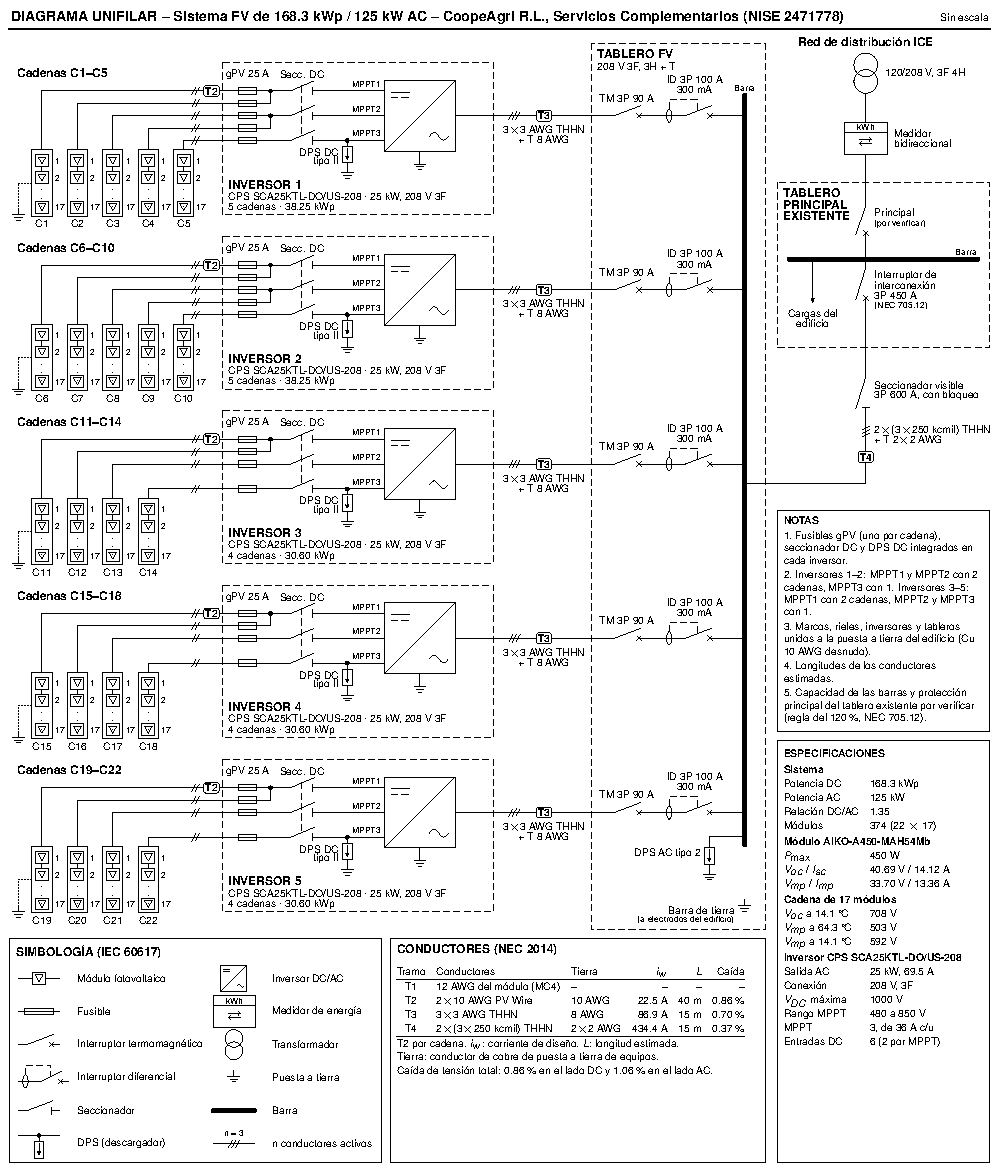
\includegraphics[width=\textwidth]{unifilar.pdf}
\caption{Diagrama unifilar del sistema fotovoltaico propuesto (\SI{168.3}{kWp} / \SI{125}{kW} AC), con simbología IEC 60617.}
\label{fig:unifilar}
\end{figure*}
